
\documentclass[12pt]{article}
\usepackage{vmargin,url,hyperref,booktabs,graphicx,rotating}
\usepackage[authoryear,round]{natbib}

\setpapersize{USletter}                 % use USletter paper
\setmarginsrb{1in}{1in}{1in}{1in}{0pt}{0pt}{\footheight}{\footskip}

\hypersetup{  
  hyperindex,%
  colorlinks,%
  linktocpage,%
  plainpages=false,%
  linkcolor=DarkBlue,%
  citecolor=DarkBlue,%
  urlcolor=DarkBlue,%
  pdfstartview=Fit,%
  pdfview={XYZ null null null}%
}
\RequirePackage{color}
\definecolor{Red}{rgb}{0.7,0,0}
\definecolor{Blue}{rgb}{0,0,0.8}
\definecolor{DarkBlue}{rgb}{0.1,0.1,0.4}
\definecolor{DarkGrey}{rgb}{0.15,0.15,0.15}

%% from jss.cls
\let\code=\texttt
\let\proglang=\textsf
\newcommand{\pkg}[1]{{\normalfont\fontseries{b}\selectfont #1}}

%% shortcuts
\newcommand{\diehard}{\textrm{diehard}}

%% 

\usepackage{/usr/lib/R/share/texmf/Sweave}
\begin{document}


%\VignetteIndexEntry{RDieHarder}
%\VignetteDepends{RDieHarder}
%\VignetteKeywords{random number generator, tests}
%\VignettePackage{RDieHarder}

\setkeys{Gin}{width=0.6\textwidth}


\title{\pkg{RDieHarder}: An R interface to the DieHarder suite of Random
  Number Generator Tests}
\author{\href{http://dirk.eddelbuettel.com}{Dirk Eddelbuettel} \\ 
  Debian \\ \url{edd@debian.org} 
  \and
  \href{http://www.phy.duke.edu/~rgb}{Robert G. Brown} \\ 
  Physics, Duke University \\ \url{rgb@phy.duke.edu} }
\date{May 2007}

\maketitle

\begin{abstract}
  \noindent The \pkg{RDieHarder} package provides the R language and
  environment with access to the DieHarder suite of tests for random number
  generators (RNGs).  It allows interactive test of random numbers generators
  directly from R, with further analysis in R of data generated by DieHarder.

  This paper describes the background and motivation of DieHarder, the
  RDieHarder package, shows two simple examples, and discusses current
  limitations and possible extensions left for future work.
\end{abstract}

\section{Introduction}

Random number generators are critically important for computational
statistics.  Simulation methods are becoming ever more common for estimation;
Monte Carlo Markov Chain is but one approach. Also, simulation methods such
as the Bootstrap have long been used in inference and are becoming a standard
part of a rigorous analysis.  As random number generators are at the heart of 
the simulation-based methods used throughout statistical computing, `good'
random numbers are therefore a crucial aspect of a statistical, or
quantitative, computing environment.  However, there are very few tools that
allow us to separate `good' from `bad' random number generators.

Based on work that started with the \pkg{random} package
\citep{Eddelbuettel:random:2007} (which provides functions that access a
non-deterministic random number generator (NDRNG) based on a physical source
of randomness), we wanted to compare the particular NDRNG to the RNGs
implemented in GNU R \citep{RCore:R:2007} itself, as well as to several RNGs
from the GNU GSL \citep{gsl:2007}, a general-purpose scientific computing
library.  Such a comparison is possible with the \textsl{dieharder} test
suite by \cite{Brown:dieharder:2007} which extends the \textsl{diehard} test
suite by Marsaglia.  Extending on this work, we became interested in making
\textsl{dieharder} directly accessible from GNU R. The \pkg{RDieHarder}
package presented here allows such access.

This paper is organized as follows. Section 2 describes the history and
design of the dieharder suite.  Section 3 describes the \pkg{RDieHarder}
package facilities. Section 4 is a simple case study examining the six
generators built into R.  Section 5 discusses current limitations and
possible extensions before section 6 concludes.


\section{DieHarder}

DieHarder is described at length in \cite{Brown:dieharderpaper:2006}.  Due
to space limitations, this section cannot provide as much detail and will
cover only a few key aspects of the DieHarder suite.

\subsection{Diehard}
Dieharder reimplements and extends George Marsaglia's \textsl{Diehard Battery
  of Tests of Randomness} \citep{Marsaglia:1996}. Due to both its robust
performance over a wide variety of RNGs, as well as an ability to discern
numerous RNGs as weak, Diehard has become something close to a `gold standard'
for assessing RNGs.

However, there are a number of drawbacks with the existing Diehard test
battery code and implementation.  First, Marsaglia undertook a large
amount of the original work a number of years ago when computing resources
were, compared to today's standards, moderately limited. Second, neither the
Fortran nor the (translated) C sources are particularly well documented, or
commented. Third, the library design is not modular in a way that
encourages good software engineering. Fourth, and last but not least, no
licensing statement is provided with the sources or on the support website.

This lead one of the authors of this paper (rgb) to a multi-year effort of
rewriting the existing tests from DieHard in a) standard C in a modular and
extensible format, along with extensive comments, and to b) relicense it
under the common and understood GNU GPL license (that is also used for GSL,
R, the Linux kernel, and numerous other projects) allowing for wider use.
Moreover, new tests from NIST were added (see next subsection) and some
genuinely new tests were developed (see below).


\subsection{STS}

The National Institute of Standards and Technology (NIST) has developed its
own test suite, the 'Statistical Test Suite' (STS). These tests are focussed
on bit-level tests of randomness and bit sequences.   

\marginpar{TODO: expand}
Currently, three tests based on the STS suite are provided by DieHarder:
\textsl{STS Monobit}, \textsl{STS Runs} and \textsl{STS Block}. 

\subsection{RGB extensions}

\marginpar{TODO: expand}
Three new tests have been developed by rgb. A fourth 'test' is a timing
function: for many contexts, not only do the mathematical properties of a
generator matter, but so does computational cost measured in computing time
that is required for a number of draws.  

\subsection{Basic methodology}

Let us suppose a random number generator can provides a sequence of $N$
uniform draws from the range $[0, 1)$. As the number of draws increases, the
mean of the sum of all these values should, under the null hypothesis of a
proper generator, converge closer and closer to $\mu = N / 2$. Each of these
$N$ draws forms one experiment.  If $N$ is sufficiently large, then the means
of all experiments should be normally distributed with a standard deviation
of $\sigma = \sqrt{ N / 12}$. Given this asymptotic result, we can, for any
given experiment $i \in 1, \ldots, M$ transform the given sum $x_i$ of $N$
draws into a probability value $p_i$ using the inverse normal
distribution.\footnote{Running \code{print(quantile(pnorm( replicate(M,
    (sum(runif(N)) - N/2) / sqrt(N/12)) ), seq(0, 1, by=0.1) )*100,
    digits=2)} performs a Monte Carlo simulation of $M$ experiments using $N$
  uniform deviates to illustrate this. Suitable values are e.g. \code{N <-
    1000; M <- 500}.}

The key insight is that, under the null hypothesis of a perfect generator,
these $p_i$ values should be uniformly distributed. Using our set of $M$
probability values, we can compute one 'meta-test' of whether we can reject
the null of a perfect generator by rejecting that our $M$ probability values
are not uniformly distributed. One suitable test is for example the
non-parametric Kolmogorov-Smirnov (KS) statistic.  Dieharder uses the Kuiper
variant \marginpar{Reference?} of the KS test which uses the combination $D_+
+ D_-$ of the maximum and minimum distance to the alternative distribution,
instead of using just one of these as in the case of the KS test.  This renders
the test more sensitive across the entire test region.

\subsection{GSL framework}

DieHarder is primarily focussed on tests for RNGs. Re-implementing RNGs in
order to supply input to the tests is therefore not an objective of the
library.  The GNU Scientific Library (GSL), on the other hand, provides 
over 1000 mathematical functions, including a large number of random number
generators.  Using the GSL 1.9.0 release, the following generators
are defined\footnote{This is based on the trailing term in each identifier
  defined in \texttt{/usr/include/gsl/gsl\_rng.h}.}:
\begin{quote}
  \small
  \texttt{borosh13 coveyou cmrg
    fishman18 fishman20 fishman2x gfsr4 knuthran knuthran2 knuthran2002
    lecuyer21 minstd mrg mt19937 mt19937\_1999 mt19937\_1998 r250 ran0 ran1
    ran2 ran3 rand rand48 random128\_bsd random128\_glibc2 random128\_libc5
    random256\_bsd random256\_glibc2 random256\_libc5 random32\_bsd
    random32\_glibc2 random32\_libc5 random64\_bsd random64\_glibc2
    random64\_libc5 random8\_bsd random8\_glibc2 random8\_libc5 random\_bsd
    random\_glibc2 random\_libc5 randu ranf ranlux ranlux389 ranlxd1 ranlxd2
    ranlxs0 ranlxs1 ranlxs2 ranmar slatec taus taus2 taus113 transputer tt800
    uni uni32 vax waterman14 zuf} 
\end{quote}
The GNU GSL, a well-known and readily available library of high quality,
therefore provides a natural fit for DieHarder. Consequently, all of these
are generators are also available in DieHarder. DieHarder uses a standardized
interface in which a generator is selected, parameterized as needed and the
called via the external GSL library against which DieHarder is linked.

Beyond these GSL generators, DieHarder also provides two generators based on
the `devices' \texttt{/dev/random} and \texttt{/dev/urandom} that are
commonly available on Unix. They provide non-deterministic random-numbers
based on entropy generated by the operating system. DieHarder also offers a
text and a raw file input generators. Lastly, a new algorithmic generator
named 'ca' that is based on cellular automata has recently been added as well.

\subsection{R random number generators}

To assess the quality of the non-deterministic RNG provided in the GNU R
add-on package \pkg{random}, benchmark comparisons with the generators
provided by the R language and environment have been a natural choice. To
this end, one of the authors (edd) ported the R generator code (taken from R
2.4.0) to the GNU GSL random number generator framework used by DieHarder.
\marginpar{TODO: use R sources from R 2.5.0} This allows a direct comparison
of the \pkg{random} generator with those it complements in R.

It then follows somewhat naturally that the other generators available in
DieHarder, as well as the DieHarder tests, should also be available in R.
This provided the motivation for the R package presented here.

\subsection{Source code and building DieHarder} 

Recent versions of DieHarder use the GNU autotools. On Unix system,
the steps required to build and install DieHarder should only be the familiar
steps \texttt{configure; make; sudo make install}. 

For Debian, initial packages have been provided and are currently available
at \url{http://dirk.eddelbuettel.com/code/tmp}.  Within due course, these
packages should be uploaded to Debian, and thus become part of the next
Debian (and Ubuntu) releases.

On Windows computers and other systems, manual builds should also be possible
given that the source code is comprised only of standard C code. 

\section{RDieHarder}

The RDieHarder package provides one key function: \texttt{dieharder}.  It can
be called with several arguments. The first one is the name of the random
number generator, and the second one is the name of the test to be applied.
For both options, the textual arguments are matched against internal vectors
to obtain a numeric argument index; alternatively the index could be supplied
directly. The remaining arguments (currently) permit to set the number of
samples (i.e.~the number of experiments run, and thus the sample size for the
final Kolmogorov-Smirnov test), the random number generator seed and whether
or not verbose operation is desired.

The returned object is of class \texttt{dieharder}, inheriting from the
standard class \texttt{htest} common for all hypothesis tests.  The standard
print method for \texttt{htest} is used; however not all possible slots are
being filled (as there is for example no choice of alternative hypothesis).

A custom summary method is provided that also computes the Kolmogorov-Smirnov
and Wilcoxon tests in R and displays a simple stem-and-leaf plot.  Lastly, a
custom plot method shows both a histogram and kernel density estimate, as
well as the empirical cumulative distribution function.


\section{Case Study: Testing RNGs in GNU R}

A simple example of using RDieHarder is provided in the examples section of
the help page. One simply calls the \texttt{dieharder} function using the
default arguments, invokes a summary (which we omit here due to space
constraints) and then calls plot on the object. This shown below.

\begin{center}
\begin{footnotesize}
%
\begin{Schunk}
\begin{Sinput}
> dh <- dieharder("mt19937", "2dsphere", seed = 12345)
> dh
\end{Sinput}
\begin{Soutput}
	Diehard Minimum Distance (2d Circle) Test

data:  Created by RNG `mt19937' with seed=12345, sample of size 100 
p-value = 0.136
\end{Soutput}
\begin{Sinput}
> plot(dh)
\end{Sinput}
\end{Schunk}
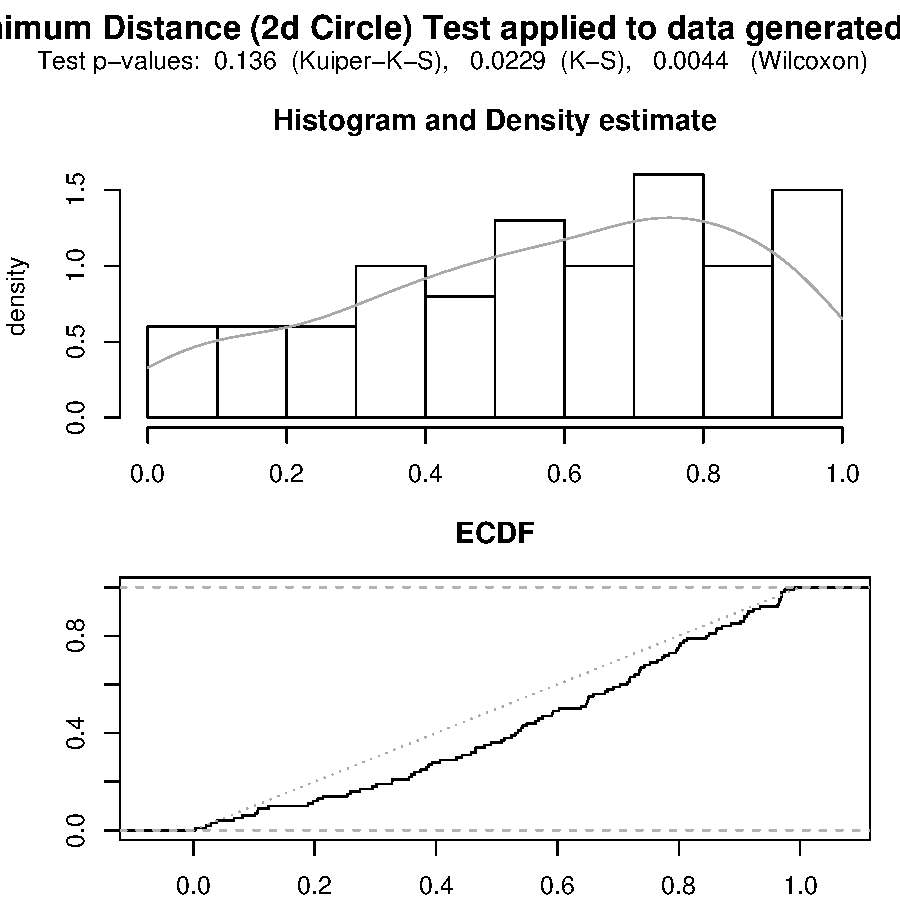
\includegraphics{RDieHarder-rd-example}
\begin{Schunk}
\begin{Sinput}
> dh1 <- dieharder("r250", "2dsphere", seed = 12345)
> dh1
\end{Sinput}
\begin{Soutput}
	Diehard Minimum Distance (2d Circle) Test

data:  Created by RNG `r250' with seed=12345, sample of size 100 
p-value = 0.7626
\end{Soutput}
\begin{Sinput}
> plot(dh1)
\end{Sinput}
\end{Schunk}
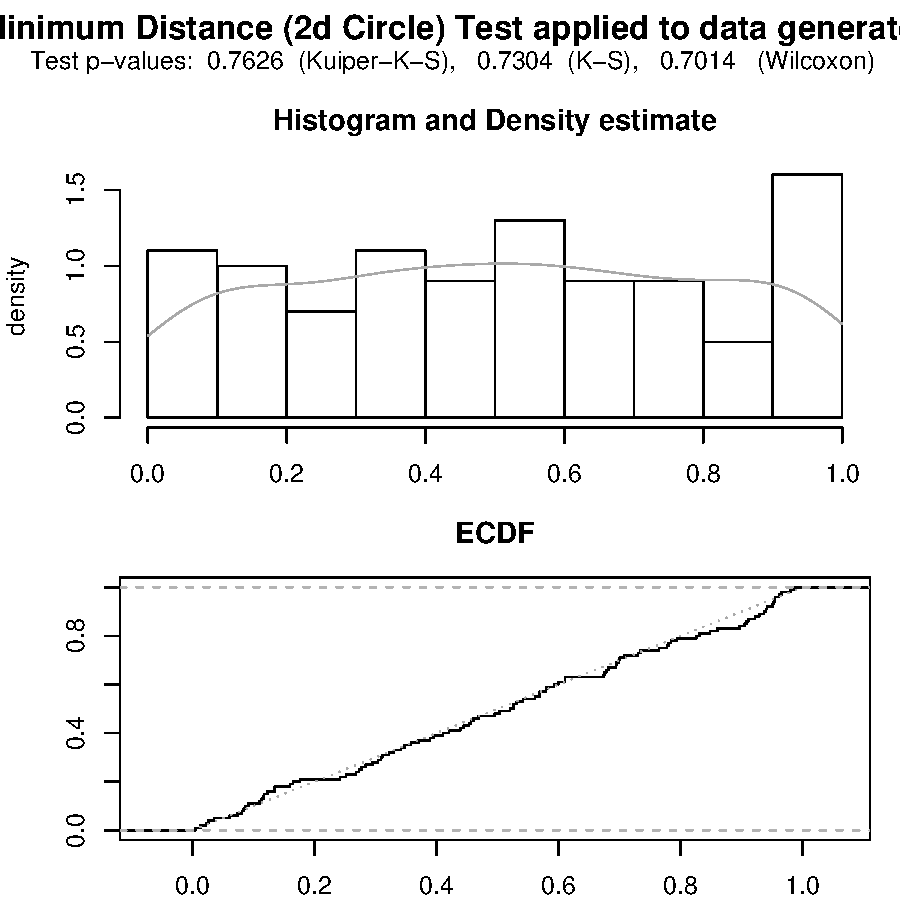
\includegraphics{RDieHarder-rd-example1}
% 
\end{footnotesize}
\end{center}

A more complete example follows below.  We define a short character vector
containing the names of the six R RNGs, apply the \texttt{dieharder} function to
each of these, and then visualize the resulting $p$-values in simple qqplot.

\begin{center}
  \begin{footnotesize}
%
\begin{Schunk}
\begin{Sinput}
> rngs <- c("R_wichmann_hill", "R_marsaglia_multic", "R_super_duper", 
+     "R_mersenne_twister", "R_knuth_taocp", "R_knuth_taocp2")
> rl <- lapply(rngs, function(rng) dieharder(rng, "runs", seed = 12345))
> oldpar <- par(mfrow = c(2, 3), mar = c(2, 3, 3, 1))
> invisible(lapply(rl, function(res) {
+     qqplot(res$data, seq(0, 1, length.out = length(res$data)), 
+         main = paste(res$generator, ":", round(res$p.value, digits = 4)), 
+         ylab = "", type = "S")
+     abline(0, 1, col = "gray")
+ }))
> par(oldpar)
\end{Sinput}
\end{Schunk}
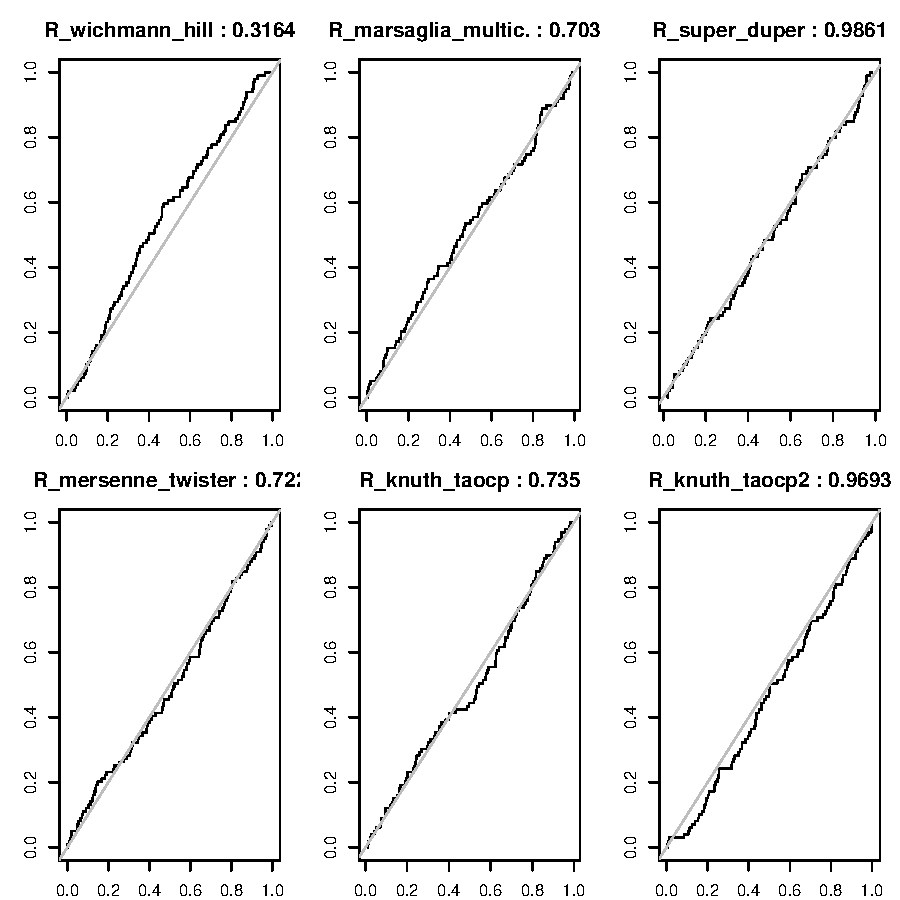
\includegraphics{RDieHarder-r-rngs}
% 
\end{footnotesize}
\end{center}

All six generators provide $p$-value plots that are close to the ideal
theoretical outcome (shown in gray). Unsurprisingly, $p$-values for the
Kuiper KS test also show no support for rejecting these generators.


\section{Current Limitations and Future Research}

The implementation of RDieHarder presented here leaves a number of avenues
for future improvement and research.  Some of these pertain to dieharder
itself -- adding new, more sophisticated, more systematic tests
including those from the STS suite and tests that probe bitlevel
randomness in unique new ways.  Others pertain more to the integration
of dieharder with R, which is the topic of this work.

Not all of dieharder's features are yet supported in this initial port.
In the near future we expect to add code to deal with tests that support
extra parameters, or that return more than one p-value per instance of a
test.  Ultimately, RDieHarder should support the full set of options of
the the command-line version of dieharder.

There is no direct interface from the R generators to the RLibDieharder
module for evaluation; rather, the 'ported' R generators are called from the
libdieharder library. This could introduce coding/porting errors, and also
prevents the direct use of user-added generators that R supports. It would be
worthwhile to overcome this by directly letting \pkg{RDieHarder} call back
into R to generate draws. On the other hand, the current setup corresponds
more closely to the command-line version of DieHarder.

Next, the R generators in DieHarder may need to be updated to the 2.5.0
code. The GSL RNGs provided by libdieharder may as well be exported to R via
\pkg{RDieHarder} given that the GSL library is already linked in.
Indeed, it would be worthwhile to {\em integrate} the two projects and
both avoid needless code duplication and ensure even more eyes checking
both the quality and accuracy of the code in both.

It could be useful to also build RDieHarder with an `embedded' libdieharder
rather than relying on an externally installed libdieharder. This may make
it easier to build RDieHarder for systems without libdieharder (and on
Windows).  Likewise, it is possible to reorganize the dieharder front-end
code into a common library to avoid duplication of code with RDieHarder.

Lastly, on the statistical side, an empirical analysis of size/power
between KS, Wilcoxon and other alternatives for generating a final
p-value from the vector of p-values returned from dieharder tests
suggests itself. Similarly, empirical comparisons between the resolving
power of the various tests (some of which may not actually be terribly
useful in the sense that they yield new information about the failure
modes of any given RNG) could be undertaken.  Lastly, there is always
room for new generators, new tests, and new visualizations.

One thing that one should remember while experimenting with dieharder is
that there really is no such thing as a {\em random} number {\em
generator}.  It is therefore likely that {\em all} RNGs will fail any
given (valid) test if one cranks up the ``resolution'' up high enough by
accumulating enough samples per p-value, enough p-values per run.  

It is also true that a number of Marsaglia's tests have target
distributions that were computed empirically by simulation (with the
best RNGs and computers available at the time).  Here one has to
similarly remember that one can do in a few hours of work what it would
have taken him months if not years of simulation to equal back when the
target statistics were evaluated.  It is by no means unlikely that a
``problem'' that dieharder eventually resolves is not not the quality of
the RNG but rather the accuracy of the target statistics.

These are some of the things that are a matter for future research
to decide.  A major motivation for writing dieharder, and making it open
source, and integrating it with $R$, is to facilitate precisely this
sort of research in an easy to use, consistent testing framework.  We
{\em welcome} the critical eyes and constructive suggestions of the
statstical community and invite their participation in examining the
code and algorithms used in dieharder.

\section{Conclusion}

The \pkg{RDieHarder} package presented here introduces several new features.
First, it makes the DieHarder suite \citep{Brown:dieharder:2007} available
for interactive use from the GNU R environment. Second, it also exports
DieHarder results directly to R for further analysis and visualization.
Third, it adds adds additional RNGs from GNU R to those from GNU GSL that
were already testable in DieHarder. Fourth, it provides a re-distribution of
the DieHarder `test engine' via GNU R.

\bibliographystyle{plainnat}
\bibliography{RDieHarder}

\end{document}
